\documentclass{article}
\usepackage{graphicx}
\usepackage[margin=1.5cm]{geometry}
\usepackage{amsmath}

\begin{document}

\title{Friday Reading Assessment: Unit 0, Review and Charge}
\author{Prof. Jordan C. Hanson}

\maketitle

\section{Review}

\begin{enumerate}
\item Suppose the velocity of a system increases by a factor of 4.  By what factor will the \textit{kinetic energy} of a system increase?
\begin{itemize}
\item A: 4
\item B: 8
\item C: 16
\item D: 32
\end{itemize}
\end{enumerate}

\section{Charge}

\begin{enumerate}
\item The balloon in Fig. \ref{fig:balloon} can be rubbed on the sweater to retain negative charge.  The balloon pulls negative charges from the sweater, and is released in between the wall and the sweater.  In which direction does it accelerate?  Why? \\ \vspace{2cm}
\begin{figure}
\centering
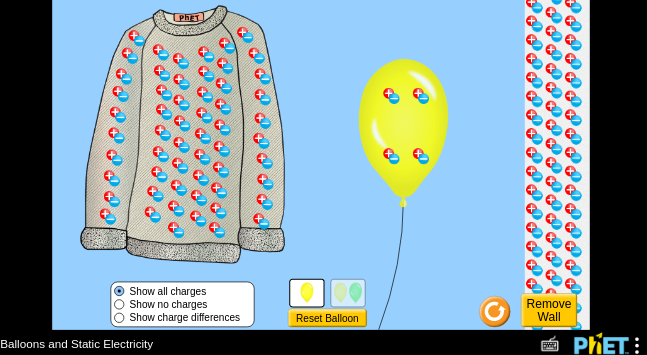
\includegraphics[width=0.5\textwidth]{balloon.png}
\caption{\label{fig:balloon} A neutral balloon can be rubbed on a neutral sweater and retain negative charge.}
\end{figure}
\item Suppose a chemical process in a solution removes one electron per atom of one type of molecule, and adds it to another.  Is charge conserved for each type of molecule?  What about the whole system?  Why or why not?  (Think of something rusting).
\end{enumerate}

\end{document}
